\section{Base de données}

\subsection{Choix du type de modélisation}

Concernant le stockage des données, nous avions plusieurs choix:

\begin{itemize}
	\item écrire dans des fichiers;
	\item installer une base de données sur un serveur distant;
	\item installer une base de données sur un serveur local à la machine;
	\item installer une base de données sans serveur, en interne au logiciel.
\end{itemize}

\paragraph{}

Pour éviter d’utiliser un système de base de données, nous aurions pu choisir d’écrire les données que l’on voudrait sauvegarder directement dans des fichiers. Cependant, cette façon de sauvegarder les données n’est pas très “propre” et est compliquée à structurer. C’est pour cette raison que nous nous sommes plutôt dirigé vers un Système de Gestion de Bases de Données (SGBD).

\paragraph{}

Utiliser un serveur distant sur lequel on installerait une base de données était notre première idée. Cependant, ce système possède un inconvénient majeur qui est que notre application aurait besoin d’une connexion internet et d’un serveur pour fonctionner. Cette contrainte ajoutant plus de complexité que nécessaire, nous n'utiliserons pas de serveur distant.
Utiliser un serveur local résoudrait le problème de la connexion internet mais il faudrait tout de même faire tourner un serveur local sur la machine qui exécute le logiciel.

\paragraph{}

La solution que nous avons retenue est l’utilisation d’une base de donnée intégrée à l’application. Ainsi, la création et la manipulation de la base sera plus simple. Le principal inconvénient de ce type de base de données est qu’on ne peut pas y accéder à plusieurs. Seul l’utilisateur du logiciel a accès aux données qu’il manipule.
Dans une amélioration possible du projet, on pourrait imaginer installer la base de données sur un serveur externe pour autoriser la multi-utilisation. Cette amélioration n’étant pas très compliquée, il sera possible de la faire en fin de projet.

\paragraph{}

Il existe de nombreux SGBD mais pour une base de données intégrée SQLite nous semble être le meilleur choix. En effet, il est open-source, gratuit et est spécifiquement destiné à être utilisé comme SGBD intégré à un logiciel. De plus, il est simple d’utilisation car il existe un Framework Java permettant de le manipuler simplement.

\subsection{Objectifs de la BDD}

Le principal objectif de la base de données est de pouvoir stocker les données traitées par notre logiciel. Ainsi il doit être possible de pouvoir stocker des imagettes associées à leur transcription (vérité terrain). On devra également pouvoir stocker les données obtenues par le système de reconnaissance d’écriture manuscrite qui aura été entraîné grâce à la base d’apprentissage que notre logiciel lui aura fourni. Ainsi il faudra aussi stocker des imagettes associées à leur transcription générée par le reconnaisseur. 

\paragraph{}

En plus de stocker les données, la partie base de données devra pouvoir communiquer facilement avec les autres blocs de notre logiciel (IHM et préparateur de données). Le fait que nous utilisions SQLite et son framework Java va nous permettre d’implémenter des méthodes Java pour accéder et manipuler simplement les données présentes dans la base. L’objectif de l’équipe qui développe la base de donnée est donc de la modéliser, la construire et de fournir une bibliothèque Java qui pourra être utilisée par le reste de l’équipe. Le but de cette bibliothèque est d’éviter aux autres équipes d’avoir à manipuler du SQL dans leur code Scala. Java étant interopérable avec Scala, le fait de la développer en Java ne posera aucun problème pour le reste du projet.

\subsection{Concernant la bibliothèque}

La bibliothèque que nous devons implémenter contiendra ainsi des méthodes dont le but est de faire le lien entre la partie base de données et les autres blocs du logiciel. Parmi ces méthodes nous retrouverons ainsi des procédés pour accéder aux données (SELECT en SQL), modifier les données (UPDATE en SQL), insérer de nouvelles données dans la base (INSERT INTO en SQL) ou encore supprimer des données de la base (DELETE en SQL). Ces méthodes devront être implémentées pour chaque table de la base de données.

\subsection{Modélisation}

Voici la manière dont nous avons modélisé la base de données :

\paragraph{}

\begin{mdframed}[frametitle={Figure 6 : Modèle entité association de la Base de données}, innerbottommargin=10]
\begin{center}
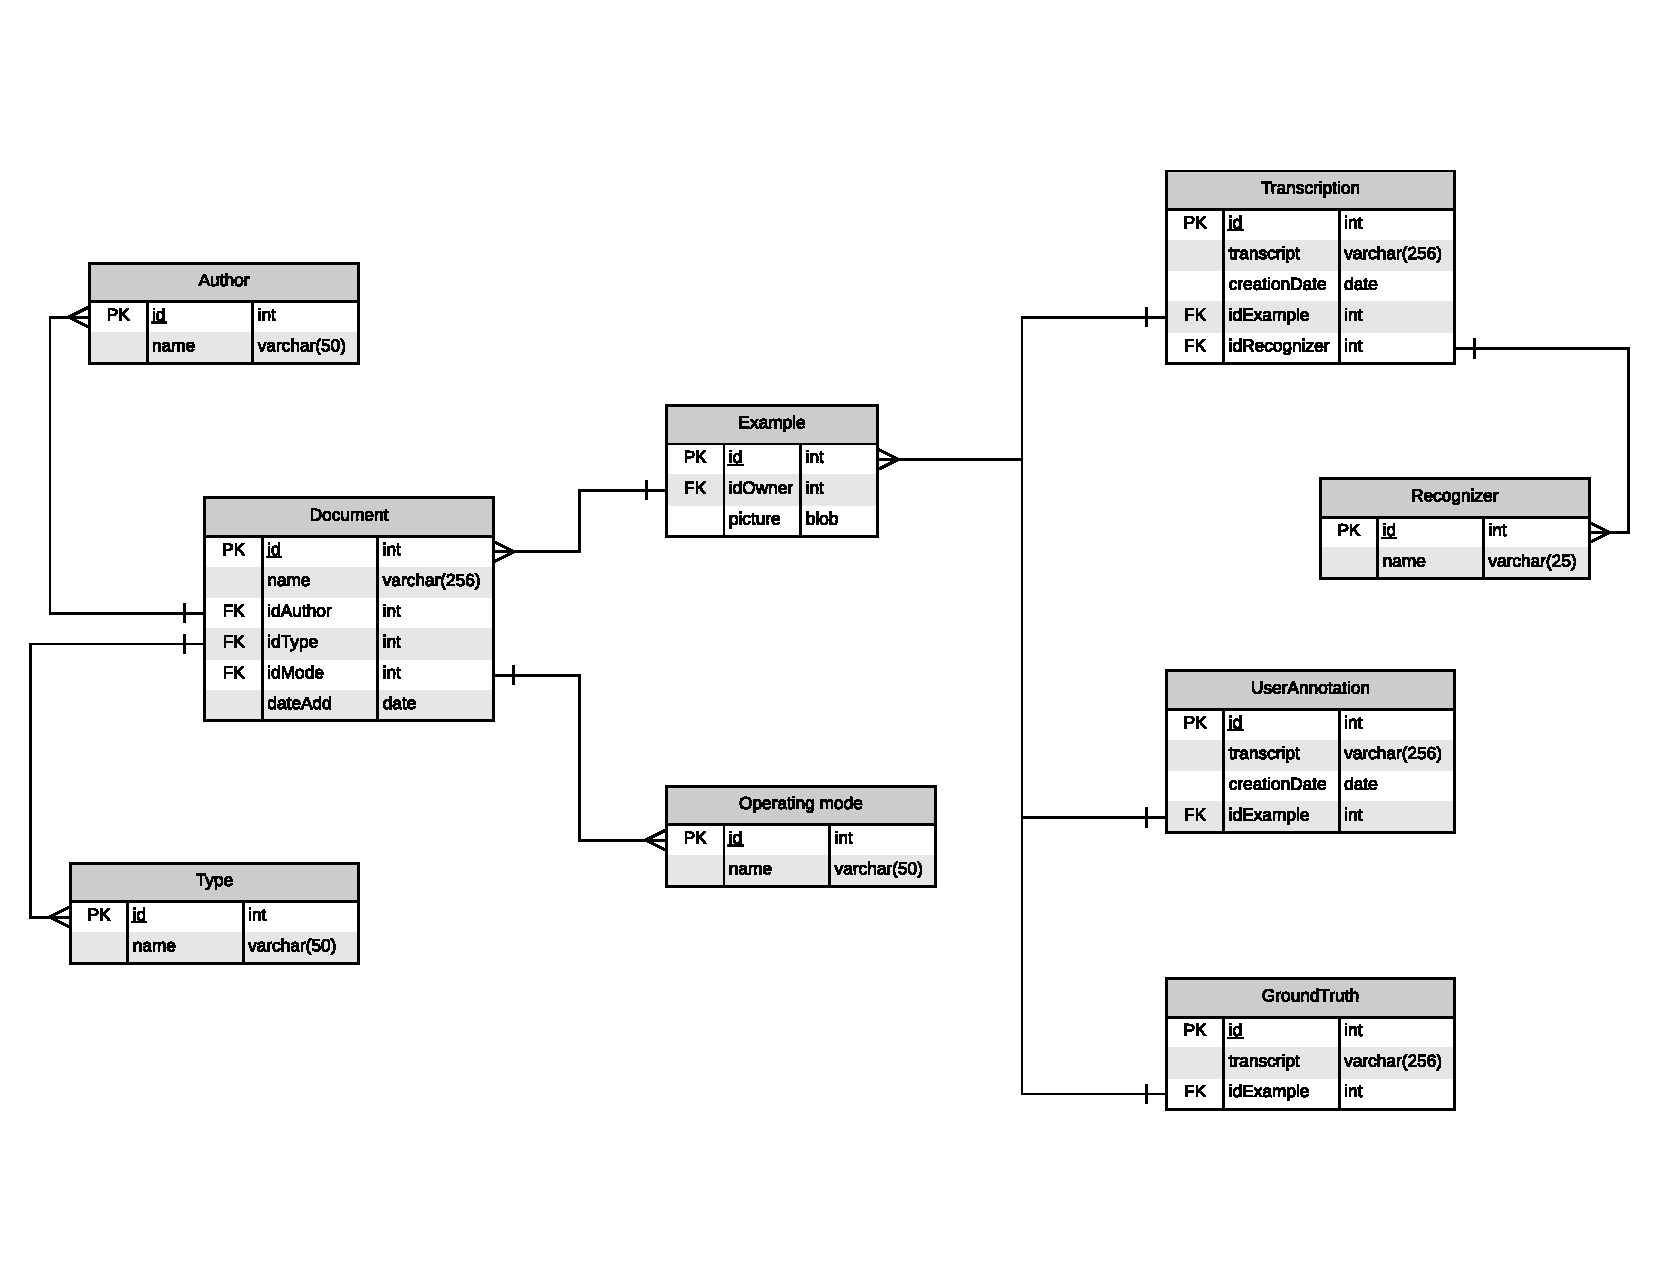
\includegraphics[width=\linewidth]{Modele_entite_association.pdf}
\end{center}
\end{mdframed}

\paragraph{}

Les tables Author, Type et Operating Mode permettent de stocker les informations concerant les auteurs des documents, le type des documents ainsi que le mode dans lequel on se trouve (mode apprentissage ou mode évaluation).
La table Document contient toutes les informations concernant un document. A savoir son nom, son auteur, son type, le mode auquel il appartient ainsi que sa date d’ajout à la base.

Nos imagettes seront stockées dans des dossiers à côté de la base de données. Elles seront donc référencées par la base de donnée grâce à leur chemin (par exemple “/home/MesImagettes/imagette1.jpg”) dans la table Example. Cette table contient en plus une référence vers le document d’origine.

\paragraph{}

Les trois tables suivantes (Transcription, UserAnnotation, GroundTruth) servent à lier les imagettes avec leur transcription. Dans la table GroundTruth, on enregistre l’id de l’imagette ainsi que sa vérité-terrain. Dans la table UserAnnotation, on enregistre la même chose mais, en plus, la date de création de cette vérité-terrain qui aura été ajoutée par un utilisateur. Enfin, dans la table Transcription, on enregistre les mêmes informations que dans la table UserAnnotation sauf que, cette fois-ci, la transcription aura été donnée par un reconnaisseur d’écriture manuscrite représenté dans la table Recognizer.








